\documentclass[border=3mm]{standalone}

\usepackage{xcolor} % before tikz or tkz-euclide if necessary
\usepackage{tikz}
\usepackage{tkz-euclide} % no need to load TikZ
\usepackage{multirow}
\usetikzlibrary{babel} %if there are problems with the active characters
\begin{document}
	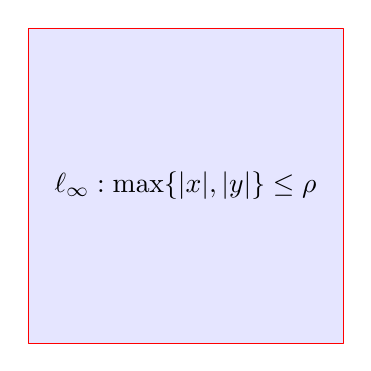
\begin{tikzpicture}
		%\hspace{-1cm}
		\tkzInit[xmax=2,ymax=3,xmin=-2.5,ymin=-3]
		\tkzDrawXY[label={}]
		\tkzDefPoint(-2,-2){K}
		\tkzDefShiftPoint[K](0:4){M}
		\tkzDefSquare(K,M)\tkzGetPoints{N}{O}
		\tkzDrawPolygon[color=red,fill=blue!10!white](K,M,N,O)
		 \node[draw=none] at (0,0) {$\ell_\infty: \max\{ |x|,|y|\}\le \rho$};
	\end{tikzpicture}
	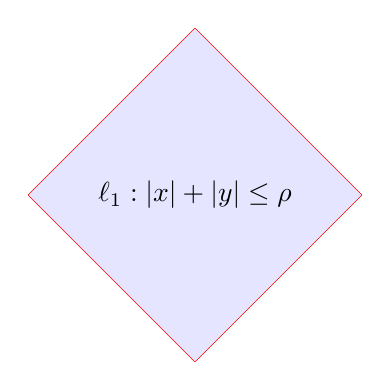
\begin{tikzpicture}
		%\hspace{-1cm}
		\tkzInit[xmax=2.5,ymax=3,xmin=-3,ymin=-3]
		\tkzDrawXY[label={}]
		\tkzDefPoint(0,-(sqrt(18))/2){K}
		\tkzDefShiftPoint[K](45:3){M}
		\tkzDefSquare(K,M)\tkzGetPoints{N}{O}
		\tkzDrawPolygon[color=red,fill=blue!10!white](K,M,N,O)
		 \node[draw=none] at (0,0) {$\ell_1: |x|+|y| \le \rho$};
	\end{tikzpicture} 
%\hspace{1cm}
	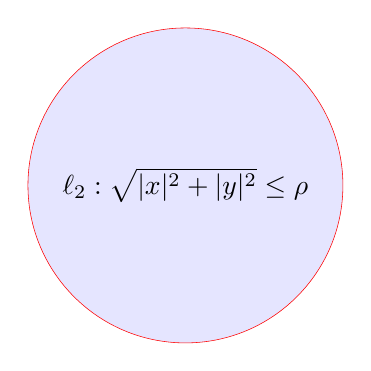
\begin{tikzpicture}
		\tkzInit[xmax=2.5,ymax=3,xmin=-2.5,ymin=-3]
		\tkzDrawXY[label={}]
		\tkzDefPoint(0,0){K}
		\tkzDefShiftPoint[K](0:2){M}
		\tkzDrawCircle[color=red,fill=blue!10!white](K,M)
		 \node[draw=none] at (0,0) {$\ell_2: \sqrt{ |x|^2+|y|^2} \le \rho$};
		
	\end{tikzpicture}

\end{document}